\documentclass[12pt]{beamer}
\usepackage{../Estilos/BeamerMAF}
\usepackage{../Estilos/ColoresLatex}
%Sección para el tema de beamer, con el theme, usercolortheme y sección de footers
\usetheme{Frankfurt}
\usecolortheme{beaver}
%\useoutertheme{default}
\setbeamercovered{invisible}
% or whatever (possibly just delete it)
\setbeamertemplate{section in toc}[sections numbered]
\setbeamertemplate{subsection in toc}[subsections numbered]
\setbeamertemplate{subsection in toc}{\leavevmode\leftskip=3.2em\rlap{\hskip-2em\inserttocsectionnumber.\inserttocsubsectionnumber}\inserttocsubsection\par}
% \setbeamercolor{section in toc}{fg=blue}
% \setbeamercolor{subsection in toc}{fg=blue}
% \setbeamercolor{frametitle}{fg=blue}
\setbeamertemplate{caption}[numbered]

\setbeamertemplate{footline}
\beamertemplatenavigationsymbolsempty
\setbeamertemplate{headline}{}


\makeatletter
% \setbeamercolor{section in foot}{bg=gray!30, fg=black!90!orange}
% \setbeamercolor{subsection in foot}{bg=blue!30!yellow, fg=red}
% \setbeamercolor{date in foot}{bg=black, fg=white}
\setbeamertemplate{footline}
{
  \leavevmode%
  \hbox{%
  \begin{beamercolorbox}[wd=.333333\paperwidth,ht=2.25ex,dp=1ex,center]{section in foot}%
    \usebeamerfont{section in foot} \insertsection
  \end{beamercolorbox}%
  \begin{beamercolorbox}[wd=.333333\paperwidth,ht=2.25ex,dp=1ex,center]{subsection in foot}%
    \usebeamerfont{subsection in foot}  \insertsubsection
  \end{beamercolorbox}%
  \begin{beamercolorbox}[wd=.333333\paperwidth,ht=2.25ex,dp=1ex,right]{date in head/foot}%
    \usebeamerfont{date in head/foot} \insertshortdate{} \hspace*{2em}
    \insertframenumber{} / \inserttotalframenumber \hspace*{2ex} 
  \end{beamercolorbox}}%
  \vskip0pt%
}







\setbeamercolor{section in foot}{bg=deepcarmine, fg=white}
\setbeamercolor{subsection in foot}{bg=flame, fg=white}
\setbeamercolor{date in foot}{bg=blue, fg=white}

\makeatletter
\setbeamertemplate{footline}
{
\leavevmode%
\hbox{%
\begin{beamercolorbox}[wd=.333333\paperwidth,ht=2.25ex,dp=1ex,center]{section in foot}%
  \usebeamerfont{section in foot} \insertsection
\end{beamercolorbox}%
\begin{beamercolorbox}[wd=.333333\paperwidth,ht=2.25ex,dp=1ex,center]{subsection in foot}%
  \usebeamerfont{subsection in foot}  \insertsubsection
\end{beamercolorbox}%
\begin{beamercolorbox}[wd=.333333\paperwidth,ht=2.25ex,dp=1ex,right]{date in head/foot}%
  \usebeamerfont{date in head/foot} \insertshortdate{} \hspace*{1.5em}
  \insertframenumber{} / \inserttotalframenumber \hspace*{2ex} 
\end{beamercolorbox}}%
\vskip0pt%
}
\makeatother
% \usefonttheme{serif}
\setbeamercolor{frametitle}{bg=lavenderblue}
\resetcounteronoverlays{saveenumi}

\AtBeginDocument{\RenewCommandCopy\qty\SI}
\ExplSyntaxOn
\msg_redirect_name:nnn { siunitx } { physics-pkg } { none }
\ExplSyntaxOff

\title{\large{Tema 4 - El átomo de hidrógeno}}
\subtitle{Funciones Especiales I}
\author{M. en C. Gustavo Contreras Mayén}

\date{14 de noviembre de 2024}

\begin{document}
\maketitle
\fontsize{14}{14}\selectfont
\spanishdecimal{.}

\section*{Contenido}
\frame[allowframebreaks]{\frametitle{Contenido} \tableofcontents[currentsection, hideallsubsections]}


\section{Partícula en un potencial central}
\frame[allowframebreaks]{\frametitle{Temas a revisar} \tableofcontents[currentsection, hideothersubsections]}
\subsection{Ecuación de Schrödinger}

%Ref. Schaum's (1998) Quantum mechanics.

\begin{frame}
\frametitle{Definiendo el problema}
El Hamiltoniano de una partícula de masa $M$ dentro de un potencial central $V (r)$ es:
\pause
\begin{align}
H = \dfrac{\vb{p}^{2}}{2 M} + V (r) = - \dfrac{\hbar^{2}}{2 M} \, \laplacian + V (r)
\label{eq:ecuacion_08_01}
\end{align}
\end{frame}
\begin{frame}
\frametitle{El Laplaciano}
Donde el Laplaciano $\laplacian$ en coordenadas esféricas es:
\pause
\begin{align}
\begin{aligned}
\laplacian &= \dfrac{1}{r} \pdv[2]{r} + \dfrac{1}{r^{2}} \bigg[ \pdv[2]{\theta} + \dfrac{1}{\sin \theta} \, \pdv{\theta} + \\[1em]
&+\dfrac{1}{\sin^{2} \theta} \, \pdv[2]{\phi} \bigg]
\end{aligned}
\label{eq:ecuacion_08_02}
\end{align}
\end{frame}
\begin{frame}
\frametitle{El momento angular}
Considerando que el momento angular se puede expresar como:
\pause
\begin{align}
\begin{aligned}
\hat{L}_{x} &=& - i \, \hbar \, \left( y \, \pdv{z} - z \, \pdv{y} \right) \\[0.5em] 
\hat{L}_{y} &=& - i \, \hbar \, \left( z \, \pdv{x} - x \, \pdv{z} \right) \\[0.5em] 
\hat{L}_{z} &=& - i \, \hbar \, \left( x \, \pdv{y} - y \, \pdv{x} \right)
\end{aligned}
\label{eq:ecuacion_01_03a}
\end{align}
\end{frame}
\begin{frame}
\frametitle{Reescribiendo el Hamiltoniano}
El Hamiltoniano $H$ lo escribimos como:
\pause
\begin{align}
H = - \dfrac{\hbar^{2}}{2 M} \, \dfrac{1}{r} \, \pdv[2]{r} + \dfrac{1}{2 M r^{2}} \, \vb{L}^{2} + V (r)
\label{eq:ecuacion_08_03}
\end{align}
Las tres componentes del operador $\vb{L}$ conmutan con $\vb{L}^{2}$, y
\end{frame}
\begin{frame}
\frametitle{Potencial de interacción}
El potencial en el átomo de hidrógeno es el potencial de interacción de tipo Coulomb entre el núcleo y el electrón.
\end{frame}
\begin{frame}
\frametitle{Potencial de interacción}
Este es un potencial radial, es decir, depende solamente de la distancia al núcleo $(r)$:
\pause
\begin{align}
V = V (r) = - \dfrac{k \, Z \, e^{2}}{r}
\label{eq:ecuacion_01}
\end{align}
donde $Z$ el número atómico (en este caso $Z=1$), $e$ es la carga del electrón y $k$ es la constante de Coulomb.
\end{frame}
\begin{frame}
\frametitle{El Hamiltoniano}
Por lo tanto el Hamiltoniano cuántico (el operador correspondiente a la energía total de sistema) se escribe como:
\pause
\begin{align}
H = - \dfrac{\hbar^{2}}{2 \, m} \, \laplacian + V (r)
\label{eq:ecuacion_02} 
\end{align}
\end{frame}
\begin{frame}
\frametitle{Sistema coordenado}
El sistema de coordenadas esféricas es el más adecuado para el problema, \pause la ecuación de Schrödinger será más fácil de resolver en este sistema.
\end{frame}
\begin{frame}
\frametitle{El operador en el sistema coordenado}
Como ya sabemos expresar el Laplaciano en este sistema, haremos uso de esa expresión:
\pause
\begin{align*}
\laplacian &= \dfrac{1}{r^{2}} \pdv{r} \left( r^{2} \pdv{\phi}{r} \right) {+} \dfrac{1}{r^{2} \sin \theta} \pdv{\theta} \left( \sin \theta \pdv{\phi}{\theta} \right) {+} \\[1em]
&+ \dfrac{1}{r^{2} \sin^{2} \theta} \pdv[2]{\phi}{\phi} 
\end{align*}
\end{frame}
\begin{frame}
\frametitle{Resolviendo de manera más sencilla}
La expresión para el Laplaciano es complicada así que buscaremos una expresión más adecuada para resolver la ecuación de Schrödinger más fácilmente.
\end{frame}

\subsection{Momento angular}

\begin{frame}
\frametitle{El momento angular}
La teoría del momento angular en mecánica cuántica es de gran importancia tanto por el número como por la variedad de sus consecuencias.
\end{frame}
\begin{frame}
\frametitle{El momento angular}
A partir de la espectroscopía rotacional, que depende del momento angular de las moléculas, se consigue información acerca de las dimensiones y formas de moléculas.
\end{frame}
\begin{frame}
\frametitle{El momento angular}
Utilizando los espectros de resonancia magnética nuclear y de resonancia paramagnética electrónica, \pause cuyo origen es el momento angular de espín de núcleos y electrones, \pause se consigue información sobre la estructura y configuración de moléculas.
\end{frame}
\begin{frame}
\frametitle{El momento angular}
El momento angular orbital de los electrones en los átomos define las forma de los orbitales atómicos los cuales, a su vez, determinan la orientación de los enlaces y la estereoquímica de las moléculas.
\end{frame}
\begin{frame}
\frametitle{El momento angular}
El momento angular de un sistema es muy importante, cuando \emph{es una constante de movimiento}, es decir, cuando se conserva, porque en este caso sirve para clasificar los niveles de energía del sistema.
\end{frame}
% \begin{frame}
% \frametitle{Operadores del momento angular}
% En mecánica cuántica los operadores de momento angular orbital son:
% \pause
% \begin{align}
% \begin{aligned}
% \hat{L}_{x} &=& - i \, \hbar \, \left( y \, \pdv{z} - z \, \pdv{y} \right) \\[0.5em] 
% \hat{L}_{y} &=& - i \, \hbar \, \left( z \, \pdv{x} - x \, \pdv{z} \right) \\[0.5em] 
% \hat{L}_{z} &=& - i \, \hbar \, \left( x \, \pdv{y} - y \, \pdv{x} \right)
% \end{aligned}
% \label{eq:ecuacion_01_03a}
% \end{align}
% \end{frame}
\begin{frame}
\frametitle{Cuadrado del momento angular}
El cuadrado del operador momento angular es tal que:
\pause
\begin{align}
\hat{L}^{2} = \hat{L} \cdot \hat{L} = \hat{L}_{x}^{2} + \hat{L}_{y}^{2} + \hat{L}_{z}^{2}
\label{eq:ecuacion_01_03b}
\end{align}
\end{frame}
\begin{frame}
\frametitle{Uso de los operadores de momento}
Para aplicar estos operadores sobre funciones del tipo $\psi(r, \theta, \phi)$ es necesario expresarlos en coordenadas polares.
\end{frame}
\begin{frame}
\frametitle{Uso de los operadores de momento}
Para ello, usamos las relaciones:
\pause
\begin{align*}
r^{2} &= x^{2} + y^{2} +z^{2} \\
\cos \theta &= \dfrac{z}{\sqrt{x^{2} + y^{2} +z^{2}}} \\
\tan \phi &= \dfrac{y}{x}
\end{align*}
\end{frame}
\begin{frame}
\frametitle{Uso de los operadores de momento}
Para luego aplicar las derivadas parciales $\pdv*{x}$, $\pdv*{y}$ y $\pdv*{z}$, se tiene:
\begin{align}
\begin{aligned}
\hat{L}_{x} &= + i\, \hbar \, \left( \sin \phi \,\pdv{\theta} + \cot \theta\, \cos \phi \, \pdv{\phi} \right) \\[0.5em] 
\hat{L}_{y} &= - i\, \hbar \, \left( \cos \phi \,\pdv{\theta} - \cot \theta\, \sin \phi \, \pdv{\phi} \right) \\[0.5em] 
\hat{L}_{z} &= - i\, \hbar \, \pdv{\phi}
\end{aligned}
\label{eq:ecuacion_01_04a}
\end{align}
\end{frame}
\begin{frame}
\frametitle{Cuadrado del operador momento}
El cuadrado del operador momento angular es:
\pause
\begin{align}
\hat{L}^{2} = - \hbar^{2} \left( \dfrac{1}{\sin \theta} \pdv{\theta} \, \sin \theta \, \pdv{\theta} + \dfrac{1}{\sin^{2} \theta} \, \pdv[2]{\phi} \right)
\label{eq:ecuacion_01_04b}
\end{align}
\end{frame}
\begin{frame}
\frametitle{Sobre el operador de momento}
Es importante notar que solo se utiliza el operador $\hat{L}^{2}$ o sus componentes, pero nunca el operador $\hat{L}$ directamente, ya que el momento angular es un vector $\va{L}$ y no un escalar.
\end{frame}
% \subsection{Constante de movimiento.}

% La condición para que el operador $\hat{O}$ represente una \emph{constante de movimiento} de un sistema es que se cumpla la relación:
% \begin{align}
% \hat{O} \, \hat{H} = \hat{H} \, \hat{O}
% \label{eq:ecuacion_01_05}
% \end{align}
% donde $\hat{H}$ es el Hamiltoniano del sistema.
% \par
% La relación anterior implica que el conmutador:
% \begin{align}
% [\hat{O}, \hat{H}] = \hat{O} \hat{H} - \hat{H} \, \hat{O}
% \label{eq:ecuacion_01_06}
% \end{align}
% vale cero.
% \par
% En efecto, cuando dos operadores conmutan, existe un conjunto de funciones que son funciones propias de los dos operadores simultáneamente. Es decir, que la misma función $\psi$ que caracteriza el estado del sistema con energía $E$:
% \begin{align*}
% \hat{H} \, \psi = E \, \psi
% \end{align*}
% también caracteriza el estado del sistema con propiedad $\hat{O}$ igual a $0$:
% \begin{align*}
% \hat{O} \, \psi = 0 \, \psi
% \end{align*}

% Dicho de otra manera, cuando el sistema se encuentra en el estado caracterizado por $\psi$, su energía es $E$ y su propiedad $\hat{O}$ es $o$. Ambos valores $E$ y $o$ son constantes mientras el sistema permanezca en el mismo estado $\psi$.
% \par
% En los casos en los que $\psi$ sea degenerada, siempre será posible construir una combinación lineal de las funciones propias correspondientes a $E$ tal que sea también función propia de $\hat{O}$.

\subsection{Reglas de conmutación}

\begin{frame}
\frametitle{Conmutación entre operadores}
Las reglas de conmutación entre los operadores de momento angular y sus componentes pueden ser deducidas fácilmente utilizando las expresiones en coordenadas cartesianas.
\end{frame}
\begin{frame}
\frametitle{Conmutación entre operadores}
Algunas identidades de los conmutadores como:
\pause
\begin{eqnarray*}
\begin{aligned}
\comm{\hat{A} + \hat{B}}{\hat{C}} &= \comm{\hat{A}}{\hat{C}} + \comm{\hat{B}}{\hat{C}} \\[0.5em]
\comm{\hat{A}^{2}}{\hat{B}} &= \comm{\hat{A}}{\hat{B}} \, \hat{A} + \hat{A} \, \comm{\hat{A}}{\hat{B}}
\end{aligned}
\end{eqnarray*}
\end{frame}
\begin{frame}
\frametitle{Conmutación entre componentes del momento}
Se cumple entonces que:
\pause
\begin{eqnarray}
\begin{aligned}
\comm{L_{x}}{L_{y}} &= i \, \hbar \, L_{z} \\[0.5em] \pause
\comm{L_{y}}{L_{z}} &= i \, \hbar \, L_{x} \\[0.5em] \pause
\comm{L_{z}}{L_{x}} &= i \, \hbar \, L_{y} \\[0.5em] \pause
\comm{\vb{L}^{2}}{L_{x}} = \comm{\vb{L}^{2}}{L_{y}} &= \comm{\vb{L}^{2}}{L_{z}} = 0
\end{aligned}
\label{eq:ecuacion_01_07}
\end{eqnarray}
\end{frame}
\begin{frame}
\frametitle{Resultado de la conmutación}
Entonces: \pause
\setbeamercolor{item projected}{bg=lava,fg=white}
\setbeamertemplate{enumerate items}{%
\usebeamercolor[bg]{item projected}%
\raisebox{1.5pt}{\colorbox{bg}{\color{fg}\footnotesize\insertenumlabel}}%
}
\begin{enumerate}[<+->]
\item $\vb{L}^{2}$ conmuta con cualquiera de sus componentes.
\item Pero las componentes no conmutan entre sí.
\end{enumerate}
\end{frame}
\begin{frame}
\frametitle{Conmutación entre momento y el Hamiltoniano}
Las propiedades de conmutación entre los operadores de momento angular orbital y el Hamiltoniano dependen del sistema y deben ser determinadas para cada problema.
\end{frame}
\begin{frame}
\frametitle{Caso particular}
Frecuentemente $\vb{L}^{2}$ y $L_{z}$ conmutan con $H$ \pause y en estos casos el módulo del momento angular y la componente sobre el eje $z$ del momento angular son constantes de movimiento.
\end{frame}
% \par
% Frecuentemente $\hat{L}^{2}$ y $\hat{L}_{z}$ conmutan con $\hat{H}$ y en estos casos el módulo del momento angular y la componente sobre el eje $z$ del momento angular son constantes de movimiento.
% \par
% Por ejemplo, en el caso de átomos hidrogenoides $\hat{H}$ y $\hat{L}_{z}$ conmutan, donde:
% \begin{align*}
% \hat{H} &= - \dfrac{\hbar^{2}}{2 \mu} \left[ \dfrac{1}{r^{2}} \pdv{r} \left( r^{2} \pdv{\phi}{r} \right) {+} \dfrac{1}{r^{2} \sin \theta} \pdv{\theta} \left( \sin \theta \pdv{\phi}{\theta} \right) {+} \right. \\[0.5em]
% &+ \left. \dfrac{1}{r^{2} \sin^{2} \theta} \pdv[2]{\phi}{\phi} \right] - \dfrac{Z \, e^{2}}{r} \\[1em]
% \hat{L}_{z} &= - i \, \hbar \, \pdv{\phi}
% \end{align*}

% Entonces:
% \begin{align*}
% \hat{H} \cdot \hat{L}_{z} &= + \dfrac{i \, \hbar^{3}}{2 \mu} \left\{ \left[ \dfrac{1}{r^{2}} \pdv{r} \left( r^{2} \pdv{\phi}{r} \right) {+} \dfrac{1}{r^{2} \sin \theta} \pdv{\theta} \left( \sin \theta \pdv{\phi}{\theta} \right) {+} \right. \right. \\[0.5em]
% &+ \left. \left. \dfrac{1}{r^{2} \sin^{2} \theta} \pdv[2]{\phi}{\phi} + \dfrac{Z \, e^{2}}{r} \right] \pdv{\phi} + \dfrac{1}{r^{2} \sin^{2} \theta} \pdv[3]{\phi}{\phi} \right\}
% \end{align*}

% Mientras que:
% \begin{align*}
% \hat{L}_{z} \cdot \hat{H}  &= + \dfrac{i \, \hbar^{3}}{2 \mu} \left\{ \pdv{\phi} \left[ \dfrac{1}{r^{2}} \pdv{r} \left( r^{2} \pdv{\phi}{r} \right) {+} \right. \right. \\[0.5em]
% &+ \dfrac{1}{r^{2} \sin \theta} \pdv{\theta} \left( \sin \theta \pdv{\phi}{\theta} \right) {+} \\[0.5em]
% &+ \left. \left. \dfrac{1}{r^{2} \sin^{2} \theta} \pdv[2]{\phi}{\phi} + \dfrac{Z \, e^{2}}{r} \right] + \dfrac{1}{r^{2} \sin^{2} \theta} \pdv[3]{\phi}{\phi} \right\}
% \end{align*}

% Sabiendo que:
% \begin{align*}
% \pdv{\phi} \, \pdv{r} = \pdv{r} \, \pdv{\phi} \\[0.5em]
% \pdv{\phi} \, \pdv{\theta} = \pdv{\theta} \, \pdv{\phi}
% \end{align*}

% Es decir, las dos expresiones son iguales, por lo que:
% \begin{align*}
% \big[ \hat{H}, \hat{L}_{z} \big] = \hat{H} \, \hat{L}_{z} - \hat{L}_{z} \, \hat{H} = 0
% \end{align*}

% En coordenadas cartesianas $\hat{L}^{2}$ depende de tres coordenadas $(x, y, z)$; en coordenadas esféricas, $\hat{L}^{2}$ depende solo de dos $(\theta, \phi)$.
% \par
% En coordenadas cartesianas una de las variables no es independiente; en coordenadas esféricas, $\hat{L}^{2}$ solo depende de los ángulos, y no de la distancia $r$.
% \par
% Los observables correspondientes a los operadores $\hat{L}_{x}$, $\hat{L}_{y}$ y $\hat{L}_{z}$, son totalmente equivalentes, lo único que cambia es su orientación con respecto al sistema de referencia. Por esta razón siempre se usa $\hat{L}_{z}$, ya que la expresión matemática de su operador es mucho más simple, depende de solo un ángulos.
% \par
% Nos apoyaremos en un resultado de la teoría de los operadores y conmutadores: : Si $\hat{A}$ y $\hat{B}$ conmutan, es decir, si  $[\hat{A}, \hat{B}] = 0$, entonces existe una solución común $\psi$  para el par de ecuaciones diferenciales correspondientes a las ecuaciones de valores propios de estos operadores, siendo $\psi$ la función propia mientras que $a$ y $b$ son los valores propios correspondientes:
% \begin{align*}
% \hat{A} \, \psi &= a \, \psi \\[0.5em]
% \hat{B} \, \psi &= b \, \psi
% \end{align*}

% Ahora bien, utilizando ese resultado y el hecho de que $[\hat{L}^{2}, \hat{L}_{z}] = 0$ podemos buscar una solución común, que escribimos como $Y(\theta, \phi)$, al par de las ecuaciones diferenciales:
% \begin{align*}
% \hat{L}_{z} \, Y(\theta, \phi) &= b \, Y(\theta, \phi) \\[0.5em]
% \hat{L}^{2} \, Y(\theta, \phi) &= c \, Y(\theta, \phi)
% \end{align*}



%Ref. Schaum's
\begin{frame}
\frametitle{Ecuación diferencial}
Tendremos la siguiente ecuación de eigenvalores:
\pause
\begin{align}
\begin{aligned}
\bigg[ - \dfrac{\hbar^{2}}{2 \mu} \, \dfrac{1}{r} \, \pdv[2]{r} (r) &+ \dfrac{\vb{L}^{2}}{2 \mu r^{2}} + V (r) \bigg] \, \psi (r, \theta, \phi) = \\[0.5em]
&= E \, \psi (r, \theta, \phi) 
\end{aligned}
\label{eq:ecuacion_08_01_02}
\end{align}
\end{frame}
\begin{frame}
\frametitle{Resultado de la conmutación}
Ya se revisó que las tres componentes de $\vb{L}$ conmutan con $\vb{L}^{2}$, por lo que también conmutan con $H$:
\pause
\begin{align}
\comm{H}{L_{x}} = \comm{H}{L_{y}} = \comm{H}{L_{z}} = 0
\label{eq:ecuacion_08_04}
\end{align}
\end{frame}
\begin{frame}
\frametitle{Observables en el átomo de hidrógeno}
Los tres observables $H$, $\vb{L}^{2}$ y $L_{z}$ conmutan, por lo que podemos buscar funciones $\psi (r, \theta, \phi)$, que también sean eigenfunciones de $\vb{L}^{2}$ y $L_{z}$.
\end{frame}
\begin{frame}
\frametitle{Componente en la dirección $z$ de $L$}
La componente $L_{z}$ del momento angular es:
\pause
\begin{align*}
L_{z} = - i \, \hbar \, \pdv{\phi}
\end{align*}
\end{frame}
\begin{frame}
\frametitle{Sistema de ecuaciones diferenciales de eigenvalores}
Ahora podremos resolver el siguiente sistema de ecuaciones diferenciales de eigenvalores:
\begin{eqnarray}
\begin{aligned}
H \, \psi (r, \theta, \phi) &= E \, \psi (r, \theta, \phi) \label{eq:ecuacion_08_05} \\[0.5em] \pause
\vb{L}^{2} \, \psi (r, \theta, \phi) &= \ell (\ell + 1) \, \hbar^{2} \, \psi (r, \theta, \phi) \label{eq:ecuacion_08_06} \\[0.5em] \pause
L_{z} \, \psi (r, \theta, \phi) &= m \, \hbar \, \psi (r, \theta, \phi) \label{eq:ecuacion_08_07}
\end{aligned}
\end{eqnarray}
\pause
y determinar aquellos estados que son eigenfunciones de $H$, $\vb{L}^{2}$ y $L_{z}$.
\end{frame}
\begin{frame}
\frametitle{Separación de variables}
Con la técnica de separación de variables, tenemos que una solución estaría dada por el producto de:
\pause
\begin{align}
\psi (r, \theta, \phi) = R (r) \, Y (\theta, \phi)
\label{eq:ecuacion_08_08}
\end{align}
\end{frame}


%Ref. Ghatak (2004) 9.3
\subsection{Problema de eigenvalores}

\begin{frame}
\frametitle{Problema de eigenvalores}
Sin pérdida de generalidad, podemos expresar nuestro problema de valores propios para $\vb{L}^{2}$ como:
\pause
\begin{align}
\vb{L}^{2} \, Y(\theta, \phi) = \lambda \, \hbar^{2} \, Y(\theta, \phi)
\label{eq:ecuacion_027}
\end{align}
\pause
donde $\lambda \, \hbar^{2}$ representan los eigenvalores de $\vb{L}^{2}$, \pause y $Y(\theta, \phi)$ corresponde a las eigenfunciones. 
\end{frame}
\begin{frame}
\frametitle{Los eigenvalores y eigenfunciones}
Veremos que:
\pause
\setbeamercolor{item projected}{bg=lava,fg=white}
\setbeamertemplate{enumerate items}{%
\usebeamercolor[bg]{item projected}%
\raisebox{1.5pt}{\colorbox{bg}{\color{fg}\footnotesize\insertenumlabel}}%
}
\begin{enumerate}[<+->]
\item $\lambda$ toma valores $\ell (\ell + 1)$ con $\ell = 0, 1, 2, \ldots$.
\item Las correspondientes eigenfunciones son los \textbf{\textcolor{cadetblue}{armónicos esféricos}}.
\end{enumerate}
\end{frame}
\begin{frame}
\frametitle{De los eigenvalores}
Para cada eigenvalor de $\ell$, habrá un orden $(2 \, \ell + 1)$ de degeneración, \pause es decir, habrá $(2 \, \ell + 1)$ eigenfunciones que corresponden al mismo eigenvalor $\ell (\ell + 1) \, \hbar^{2}$.
\end{frame}
\begin{frame}
\frametitle{Ocupando el operador momento angular}
El operador $\vb{L}^{2}$ lo sustituimos en la ec. (\ref{eq:ecuacion_027}), así que:
\pause
\begin{align}
\begin{aligned}
\dfrac{1}{\sin \theta} \pdv{\theta} \bigg[ \sin \theta \, \pdv{Y}{\theta} \bigg] &+ \dfrac{1}{\sin^{2} \theta} \, \pdv[2]{Y}{\phi} + \\[0.5em]
&+ \lambda \, Y(\theta, \phi) = 0
\end{aligned}
\end{align}
\end{frame}
\begin{frame}
\frametitle{Resolviendo la ecuación}
Para resolver esta ecuación, usamos la técnica de separación de variables.
\\
\bigskip
\pause
Proponemos una solución de la forma:
\pause
\begin{align}
Y(\theta, \phi) = \Theta(\theta) \, \Phi(\phi)
\label{eq:ecuacion_029}
\end{align}
\end{frame}
\begin{frame}
\frametitle{Avanzando en la técnica}
Que sustituimos en la expresión anterior, para luego multiplicar por:
\pause
\begin{align*}
\dfrac{\sin^{2} \theta}{Y(\theta, \phi)}
\end{align*}
\end{frame}
\begin{frame}
\frametitle{Resultado obtenido}
Entonces obtendremos:
\pause
\begin{align}
\begin{aligned}
\dfrac{\sin^{2} \theta}{\Theta} &\left[ \dfrac{1}{\sin \theta} \pdv{\theta} \, \sin \theta \, \pdv{\Theta}{\theta} + \lambda \, \Theta (\theta) \right] = \\[0.5em]
&= - \dfrac{1}{\Phi} \, \dv[2]{\Phi}{\phi} = m^{2}
\end{aligned}
\label{eq:ecuacion_030}
\end{align}
\end{frame}
\begin{frame}
\frametitle{Las variables separadas}
De hecho, las variables se han separado y hemos establecido cada lado igual a una constante positiva $m^{2}$, cuya razón quedará clara en breve.
\end{frame}
\begin{frame}
\frametitle{Ecuación resultante}
La ec. (\ref{eq:ecuacion_030}) nos da:
\pause
\begin{align*}
\dv[2]{\Phi}{\phi} + m^{2} \Phi (\phi) = 0
\end{align*}
\end{frame}
\begin{frame}
\frametitle{Solución a la ED}
Cuya solución está dada por:
\pause
\begin{align*}
\Phi(\phi) \sim e^{i m \phi}
\end{align*}
\end{frame}
\begin{frame}
\frametitle{Función univaluada}
Para que la función de onda sea univaluada, debe de ocurrir que:
\pause
\begin{align}
\Phi(\phi +  2 \, \pi) = \Phi(\phi)
\label{eq:ecuacion_031}
\end{align}
\end{frame}
\begin{frame}
\frametitle{De manera equivalente}
Que es equivalente a:
\pause
\begin{align*}
e^{2 \pi m i} = 1
\end{align*}
\end{frame}
\begin{frame}
\frametitle{Valor de la constante}
Obteniendo entonces que:
\pause
\begin{align*}
m = 0, \pm 1, \pm 2, \ldots
\end{align*}
\end{frame}
\begin{frame}
\frametitle{Elección de la constante}
En este paso se justifica que no podríamos haber establecido una constante positiva (o compleja) porque entonces la función de onda no habría sido de un solo valor.
\end{frame}
\begin{frame}
\frametitle{Las eigenfunciones}
Al identificar las funciones con un subíndice $m$, tenemos:
\pause
\begin{align}
\Phi_{m}(\phi) = \dfrac{1}{\sqrt{2 \, \pi}} \, e^{i m \phi} \hspace{1cm} m = \pm 1, \pm 2, \ldots
\label{eq:ecuacion_032}
\end{align}
\end{frame}
\begin{frame}
\frametitle{Relevancia del factor}
Donde el factor $\dfrac{1}{\sqrt{2 \, \pi}}$ asegura que:
\pause
\begin{align*}
\scaleint{6ex}_{\bs 0}^{2 \pi} \abs{\Phi_{m}(\phi)}^{2} \dd{\phi} = 1
\end{align*}
que es la condición de normalización.
\end{frame}
\begin{frame}
\frametitle{Condición de ortonormalización}
Entonces se tendrá que:
\pause
\begin{align}
\scaleint{6ex}_{\bs 0}^{2 \pi} \Phi_{\ptilde{m}}^{*}(\phi) \, \Phi_{m}(\phi) \dd{\phi} = \delta_{m \ptilde{m}}
\label{eq:ecuacion_033}
\end{align}
representa la condición de ortonormalización para $\Phi_{m}(\phi)$.
\end{frame}
\begin{frame}
\frametitle{Segunda variable}
Para la segunda ecuación $\Theta (\theta)$ (ec. \ref{eq:ecuacion_030}), tendremos que:
\pause
\begin{align}
\dfrac{1}{\sin \theta} \dv{\theta} \left( \sin \theta \, \dv{\Theta}{\theta} \right) + \left( \lambda - \dfrac{m^{2}}{\sin^{2} \theta} \right) \, \Theta (\theta) = 0
\label{eq:ecuacion_034}
\end{align}
\end{frame}
\begin{frame}
\frametitle{Cambiando la variable}
Hacemos el siguiente cambio de variable: $\cos \theta = \mu$ y $\Theta(\theta) = F(\mu)$, para obtener:
\pause
\begin{align}
\dv{\mu} \left[ (1 - \mu^{2}) \, \dv{F}{\mu} \right] + \left[ \lambda - \dfrac{m^{2}}{1 - \mu^{2}} \right] \, F(\mu) = 0
\label{eq:ecuacion_035}
\end{align}
\end{frame}
\begin{frame}
\frametitle{Resultado que depende de $m$}
Hay que considerar dos casos: $m = 0$ y $m \neq 0$.
\pause
\setbeamercolor{item projected}{bg=lava,fg=white}
\setbeamertemplate{enumerate items}{%
\usebeamercolor[bg]{item projected}%
\raisebox{1.5pt}{\colorbox{bg}{\color{fg}\footnotesize\insertenumlabel}}%
}
\begin{enumerate}[<+->]
\item Con $m = 0$, la ec. (\ref{eq:ecuacion_035}) se reduce a:
\pause
\begin{align}
(1 - \mu^{2}) \, \dv[2]{F}{\mu} - 2  \, \mu \, \dv{F}{\mu} + \lambda \, F(\mu) = 0
\label{eq:ecuacion_036}
\end{align}
\seti
\end{enumerate}
\end{frame}
\begin{frame}
\frametitle{Solución a la ED}
Las soluciones a la ec. (\ref{eq:ecuacion_036}) se conocen como los \textbf{\textcolor{blue(munsell)}{polinomios ordinarios de Legendre}} $P_{n} (x)$.
\end{frame}
\begin{frame}
\frametitle{El otro caso de $m$}
\setbeamercolor{item projected}{bg=lava,fg=white}
\setbeamertemplate{enumerate items}{%
\usebeamercolor[bg]{item projected}%
\raisebox{1.5pt}{\colorbox{bg}{\color{fg}\footnotesize\insertenumlabel}}%
}
\begin{enumerate}[<+->]
\conti
\item con $m \neq 0$: \pause El método de \enquote{fuerza bruta} para obtener $Y_{\ell m} (\theta, \phi)$ es resolver directamente la ec. (\ref{eq:ecuacion_035}).
\\
\bigskip
\pause
La solución corresponde a la función especial: \textbf{\textcolor{carmine}{polinomios asociados de Legendre}}: $P_{l}^{m} (x)$.
\end{enumerate}
\end{frame}
\begin{frame}
\frametitle{Método ocupando el momento angular}
Sin embargo, \pause la forma más sencilla y elegante de obtener las soluciones es mediante el uso de los \emph{\textcolor{darkorchid}{operadores de escalera}} del momento angular, que también revisaremos esa solución.
\end{frame}
\begin{frame}
\frametitle{Solución inicial}
Hemos llegado a plantear una ecuación diferencial para la parte angular, \pause nos falta considerar la parte radial.
\end{frame}
\begin{frame}
\frametitle{Otro par de funciones especiales}
De  la ecuación radial, se tendrán como solución:
\setbeamercolor{item projected}{bg=lava,fg=white}
\setbeamertemplate{enumerate items}{%
\usebeamercolor[bg]{item projected}%
\raisebox{1.5pt}{\colorbox{bg}{\color{fg}\footnotesize\insertenumlabel}}%
}
\begin{enumerate}[<+->]
\item \textbf{\textcolor{bole}{Polinomios asociados de Laguerre $L_{n}^{k} (r)$}}.
\item Como caso especial, los \textbf{\textcolor{darkred}{polinomios ordinarios de Laguerre $L_{n} (r)$}}.
\end{enumerate}
\end{frame}
\begin{frame}
\frametitle{Solución completa}
Para la solución completa de cualquier problema de una partícula con un potencial radial, se tiene que la función de onda es un producto de un factor radial y un armónico esférico:
\pause
\begin{align*}
\psi_{n \ell m} (r, \theta, \phi) = R_{n \ell} (r) \, Y_{\ell m} (\theta, \phi)
\end{align*}
\end{frame}

%Referencia Riley. 18.2 Funciones asociadas de Legendre

\section{Funciones asociadas de Legendre.}
\frame[allowframebreaks]{\frametitle{Temas a revisar} \tableofcontents[currentsection, hideothersubsections]}
\subsection{Definición}

\begin{frame}
\frametitle{La ecuación diferencial}
La ecuación asociada de Legendre tiene la forma:
\pause
\begin{equation}
(1 - x^{2}) \sderivada{y} - 2 \, x \, \pderivada{y} + \left[ \ell (\ell + 1) - \dfrac{m^{2}}{1 - x^{2}} \right] \, y = 0
\label{eq:ecuacion_18_28}
\end{equation}
\pause
que tiene tres puntos singulares en $x = -1, 1, \infty$, se reduce a la ecuación de Legendre (\ref{eq:ecuacion_18_01}) cuando $m = 0$.
\end{frame}
\begin{frame}
\frametitle{Naturaleza de la ED}
Se presenta en problemas de la física que involucran el operador $\nabla^{2}$, cuando se expresa en coordenadas esféricas.
\\
\bigskip
\pause
En esos casos, $- \ell \leq m \leq \ell$ y $m$ está restringida a valores enteros.
\end{frame}
\begin{frame}
\frametitle{Naturaleza de la ED}
Como en el caso de la ecuación de Legendre, la variable $x$ es el coseno del ángulo polar en coordenadas esféricas, por tanto $-1 \leq x \leq 1$.
\\
\bigskip
\pause
Cualquier solución de la ecuación \ref{eq:ecuacion_18_28}) es llamada la \textocolor{ao}{función asociada de Legendre}.
\end{frame}
\begin{frame}
\frametitle{Estudiando la ED}
El punto $x = 0$ es un punto ordinario, y del cual se pueden obtener soluciones en series de la forma:
\pause
\begin{align*}
y (x) = \nsum_{n=0} a_{n} \, x^{n}
\end{align*}
de la misma manera que se hizo para la ecuación de Legendre.
\end{frame}
\begin{frame}
\frametitle{Estudiando la ED}
En este caso, debemos de notar que si $u (x)$ es solución de la ecuación de Legendre, entonces:
\pause
\begin{equation}
y (x) = (1 -x^{2})^{\abs{m}/ 2} \dv[\abs{m}]{u}{x}
\label{eq:ecuacion_18_29}
\end{equation}
es solución a la ecuación asociada.
\end{frame}
\begin{frame}
\frametitle{Soluciones independientes}
De las dos soluciones en series linealmente independientes de la ecuación de Legendre dada por:
\pause
\begin{align*}
y_{1} (x) &= 1 - \ell (\ell + 1) \dfrac{x^{2}}{2!} + \\[0.5em]
&+ (\ell - 2)\; \ell \; (\ell + 1)\;(\ell + 3) \dfrac{x^{4}}{4!} - \ldots
\end{align*}
\end{frame}
\begin{frame}
\frametitle{Soluciones independientes}
Y por:
\pause
\begin{align*}
y_{2} (x) &= x - (\ell - 1)(\ell + 2) \dfrac{x^{3}}{3!} + \\[0.5em]
&+ (\ell - 3) (\ell - 1)(\ell + 2)(\ell + 4) \dfrac{x^{5}}{5!} - \ldots
\end{align*}
que ahora denotamos por $u_{1} (x)$ y $u_{2}(x)$.
\end{frame}
\begin{frame}
\frametitle{Soluciones independientes}
Podemos obtener dos soluciones en series linealmente independientes, $y_{1} (x)$ y $y_{2} (x)$, a la ecuación asociada mediante el uso de (\ref{eq:ecuacion_18_29}). 
\end{frame}
\begin{frame}
\frametitle{Soluciones independientes}
A partir de la discusión general de la convergencia de la series de potencias, vemos que tanto $y_{1} (x)$ como $y_{2} (x)$ también convergen para $\abs{x} < 1$.
\end{frame}
\begin{frame}
\frametitle{Solución general}
Por lo tanto la solución general de la ecuación(\ref{eq:ecuacion_18_28}) en este rango está dada por:
\pause
\begin{align*}
y(x) = c_{1} \, y_{1} (x) + c_{2} \, y_{2} (x)
\end{align*}
\end{frame}

\subsection{Asociadas de Legendre para enteros $\ell$}

\begin{frame}
\frametitle{Valores enteros}
Si $\ell$ y $m$ son ambos enteros, como suele encontrarse en varios problemas de la física, \pause entonces la solución general de la ecuación (\ref{eq:ecuacion_18_28}) se expresa por:
\pause
\begin{equation}
y (x) = c_{1} \, P_{\ell}^{m} (x) + c_{2} \, Q_{\ell}^{m} (x)
\label{eq:ecuacion_18_31}
\end{equation}
\pause
donde $P_{\ell}^{m} (x)$ y $Q_{\ell}^{m} (x)$ son las \textocolor{carmine}{funciones asociadas de Legendre de primera y segunda clase}, respectivamente.
\end{frame}
\begin{frame}
\frametitle{Valores negativos}    
Para valores no negativos de $m$, esas funciones están relacionadas a las funciones de Legendre para enteros $\ell$ mediante:
\pause
\begin{eqnarray}
\begin{aligned}
P_{\ell}^{m} (x) = (1 - x^{2})^{m/2} \, \dv[m]{P_{\ell}}{x} \\[1em] \pause
Q_{\ell}^{m} (x) = (1 - x^{2})^{m/2} \, \dv[m]{Q_{\ell}}{x}
\end{aligned}
\label{eq:ecuacion_18_32}
\end{eqnarray}
\end{frame}
\begin{frame}
\frametitle{Relación entre las funciones}
Vemos inmediatamente que, en caso necesario, las funciones asociadas de Legendre se reducen a las funciones ordinarias de Legendre cuando $m = 0$.
\end{frame}
\begin{frame}
\frametitle{Relación entre las funciones}
Dado que $m^{2}$ aparece en la ecuación asociada de Legendre (\ref{eq:ecuacion_18_28}), las funciones asociadas de Legendre para los valores negativos $m$ debe ser proporcional a la función correspondiente para valores no negativos $m$. 
\end{frame}
\begin{frame}
\frametitle{Relación entre las funciones}
La constante de proporcionalidad es una cuestión de convención.
\\
\bigskip
\pause
Para el $P_{\ell}^{m} (x) $, es habitual considerar la definición (\ref{eq:ecuacion_18_32}) como válida también para los valores negativos $m$.
\end{frame}
\begin{frame}
\frametitle{Relación entre las funciones}
Aunque la diferenciación de un número negativo no está definida, cuando $P_{\ell} (x)$ se expresa en términos de la fórmula de Rodrigues:
\pause
\begin{align*}
P_{\ell} (x) = \dfrac{1}{2^{\ell} \; \ell !} \, \dv[\ell]{x}  (x^{2} - 1)^{\ell}    
\end{align*}
este problema no se presenta para $\ell \leq m \leq \ell$. 
\end{frame}
\begin{frame}
\frametitle{Relación entre las funciones}
En este caso:
\pause
\begin{equation}
P_{\ell}^{-m} (x) = (-1)^{m} \, \dfrac{(\ell - m)!}{(\ell + m)!} \, P_{\ell}^{m} (x)
\label{eq:ecuacion_18_33}
\end{equation}
Ya que $P_{\ell}(x)$ es un polinomio de orden $\ell$, tenemos que $P_{\ell}^{m}(x) = 0$ para $\abs{m} > \ell$.
\end{frame}
\begin{frame}
\frametitle{Relación entre las funciones}
De esta definición, queda claro que $P_{\ell}^{m} (x)$ es también un polinomio de orden $\ell$ si $m$ es par, ya que contiene el factor $(1-x^{2})$ a una potencial fraccionaria si $m$ es impar.
\\
\bigskip
\pause
En cualquier caso $P_{\ell}^{m}(x)$ es regular en $x = \pm 1$.
\end{frame}
\begin{frame}
\frametitle{Funciones asociadas}
Las primeras funciones asociadas de Legendre de primera clase, se construyen fácilmente y están dadas por (se omiten los casos $m = 0$):
\end{frame}
\begin{frame}
\frametitle{Funciones asociadas}
\begin{eqnarray*}
\begin{aligned}
P_{1}^{1} (x) &= (1-x^{2})^{1/2} \\ \pause
P_{2}^{1} (x) &= 3x (1-x^{2})^{1/2}  \\ \pause
P_{2}^{2} (x) &= 3(1-x^{2})  \\ \pause
P_{3}^{1} (x) &= \frac{3}{2}(5x^{2}-1)(1-x^{2})^{1/2} \\ \pause
P_{3}^{2} (x) &= 15x (1-x^{2}) \\ \pause
P_{3}^{3} (x) &= 15 (1-x^{2})^{3/2} 
\end{aligned}
\end{eqnarray*}
\end{frame}
\begin{frame}[plain]
\begin{figure}
    \centering
    \includegraphics[scale=0.7]{Imagenes/plot_Asociados_Legendre_01.pdf}
\end{figure}
\end{frame}
\begin{frame}[plain]
\begin{figure}
    \centering
    \includegraphics[scale=0.7]{Imagenes/plot_Asociados_Legendre_02.pdf}
\end{figure}
\end{frame}
\begin{frame}[plain]
\begin{figure}
    \centering
    \includegraphics[scale=0.7]{Imagenes/plot_Asociados_Legendre_03.pdf}
\end{figure}
\end{frame}
\begin{frame}[plain]
\begin{figure}
    \centering
    \includegraphics[scale=0.7]{Imagenes/plot_Asociados_Legendre_04.pdf}
\end{figure}
\end{frame}
\begin{frame}
\frametitle{Singularidad en la función}
Debemos de mencionar que las funciones asociadas de Legendre de segunda clase $Q_{\ell}^{m} (x)$ como las $Q_{\ell}(x)$ son singulares en $x= \pm 1$.
\end{frame}

\subsection{Propiedades de \texorpdfstring{$P_{\ell}^{m}$}{P l m}}

\begin{frame}
\frametitle{Uso de un ángulo}
Cuando encontramos en problemas físicos, la variable $x$ de la ecuación asociada de Legendre (como en la ecuación ordinaria Legendre) es generalmente el coseno del ángulo polar $\theta$ en coordenadas polares esféricas.
\end{frame}
\begin{frame}
\frametitle{Uso de un ángulo}
Entonces queremos que la solución $y (x)$ sea regular en $x = \pm 1$ (correspondiente a $\theta = 0$ o $\theta = \pi$).
\end{frame}
\begin{frame}
\frametitle{Solución regular}
Para que esto ocurra, \pause se requiere que $\ell$ sea un número entero y que el coeficiente $c_{2}$ de la función $Q_{\ell}^{m} (x)$ en la ecuación (\ref{eq:ecuacion_18_31}) sea cero.
\end{frame}
\begin{frame}
\frametitle{Solución regular}
Dado que $Q_{\ell}^{m}(x)$ es singular en $x = \pm 1$, \pause con el resultado de que la solución general son múltiplos de las funciones asociadas de Legendre de primera clase $P_{\ell}^{m}(x)$.
\end{frame}

\subsection{Ortogonalidad mutua}

\begin{frame}
\frametitle{Ecuación autoadjunta}
Ya se mencionó anteriormente que la ecuación asociada de Legendre es del tipo Sturm-Liouville con:
\pause
\begin{eqnarray*}
\begin{aligned}
p &= 1 - x^{2} \\ \pause
q &= - \dfrac{m^{2}}{(1 - x^{2})} \\ \pause
\lambda &= \ell (\ell + 1) \\ \pause
w &= 1
\end{aligned}
\end{eqnarray*}
siendo su intervalo natural en $[-1,1]$.
\end{frame}
\begin{frame}
\frametitle{De la ortogonalidad}
Dado que las funciones asociadas de Legendre $P_{\ell}^{m} (x)$ son regulares en los extremos $x = \pm 1$, entonces deben de ser mutuamente ortogonales en este intervalo para un valor fijo de $m$.
\end{frame}
\begin{frame}
\frametitle{De la ortogonalidad}
Es decir:
\pause
\begin{equation}
\scaleint{6ex}_{-1}^{1} P_{\ell}^{m} (x) \, P_{k}^{m} (x) \dd{x} = 0, \hspace{1cm} \text{ si } \ell \neq k
\label{eq:ecuacion_18_36}
\end{equation}
Nótese que el valor de $m$ debe de ser el mismo en ambas funciones asociadas de Legendre para que la expresión sea válida.
\end{frame}
\begin{frame}
\frametitle{De la ortogonalidad}
La condición de normalización cuando $\ell = k$ se obtiene de la fórmula de Rodrigues:
\pause
\begin{equation}
\begin{aligned}[b]
I_{\ell m} &= \scaleint{6ex}_{-1}^{1} P_{\ell}^{m} \, (x) P_{\ell}^{m} (x) \dd{x} = \\[0.5em] \pause
&= \dfrac{2}{2 \ell + 1} \, \dfrac{(\ell +m)!}{(\ell - m)!}
\end{aligned}
\label{eq:ecuacion_18_37}
\end{equation}
\end{frame}
\begin{frame}
\frametitle{De la ortogonalidad}
Las condiciones de ortogonalidad y normalización, ecuaciones (\ref{eq:ecuacion_18_36}) y (\ref{eq:ecuacion_18_37}), respectivamente, \pause significan que la funciones asociadas de Legendre $P_{\ell}^{m}(x)$, con $m$ fija:
\end{frame}
\begin{frame}
\frametitle{Expansión de una función}
Puede utilizarse de manera similar a los polinomios de Legendre para expandir cualquier función $f (x)$ razonable en el intervalo $\abs{x} < 1$ en una serie de la forma:
\pause
\begin{equation}
f (x) = \nsum_{k=0}^{\infty} a_{m+k} \, P_{m+k}^{m} (x)
\label{eq:ecuacion_18_38}
\end{equation}
\end{frame}
\begin{frame}
\frametitle{Expansión de una función}
Donde los coeficientes están dados por:
\pause
\begin{align*}
a_{\ell} = \dfrac{2 \ell + 1}{2} \: \dfrac{(\ell - m)!}{(\ell + m)!} \scaleint{6ex}_{-1}^{1} f (x) \, P_{\ell}^{m} (x) \dd{x}
\end{align*}
\end{frame}

\subsubsection{Función generatriz}

\begin{frame}
\frametitle{La función generatriz}
La función generatriz para las funciones asociadas de Legendre, se obtienen de la combinación de su definición con la función generatriz de los polinomios de Legendre:
\pause
\begin{equation}
\begin{aligned}[b]
G (x, h) &= \dfrac{(2m)! \, (1 - x^{2})^{m/2}}{2^{m} \, m! \, (1 - 2 \, h \, x + h^{2})^{m+1/2}} = \\[0.5em] \pause
&= \nsum_{n=0}^{\infty} P_{n+m}^{m} (x) \, h^{n}
\end{aligned}
\label{eq:ecuacion_18_40}
\end{equation}
\end{frame}

\subsection{Relaciones de recurrencia}

\begin{frame}
\frametitle{Relaciones de recurrencia}
Como era de esperar, las funciones asociadas de Legendre satisfacen ciertas relaciones de recurrencia.
\\
\bigskip
\pause
De hecho, la presencia de los dos índices $n$ y $m$ significa que se puede derivar una gama mucho más amplia de relaciones de recurrencia.
\end{frame}
\begin{frame}
\frametitle{Relaciones útiles}
Presentaremos sólo cuatro de las relaciones más útiles:
\pause
\begin{eqnarray*}
\begin{aligned}
&P_{n}^{m+1} = \dfrac{2 \, m \, x}{(1-x^{2})^{1/2}} P_{n}^{m} {+} [m(m {-} 1) {-} n (n {+} 1)] \, P_{n}^{m-1} \\[0.25em] \pause
&(2 \, n {+} 1) \, x \, P_{n}^{m} = (n {+} m) \, P_{n-1}^{m} {+} (n {-} m {+} 1) \, P_{n+1}^{m} \\[0.25em] \pause
&(2 \, n {+} 1) \, (1 {-} x^{2})^{1/2} \, P_{n}^{m} = P_{n+1}^{m+1} {-} P_{n-1}^{m+1} \\[0.25em] \pause
&2 \, (1 {-} x^{2})^{1/2} \, (P_{n}^{m})^{\prime} = P_{n}^{m+1} {-} (n {+} m) \, (n {-} m {+} 1) \, P_{n}^{m-1}
\end{aligned}
\end{eqnarray*}
\end{frame}
\begin{frame}
\frametitle{Relaciones útiles}
Las relaciones de recurrencia son válidas tanto para valores negativos como positivos de $m$.
\end{frame}

\section{Armónicos esféricos}
\frame[allowframebreaks]{\frametitle{Temas a revisar} \tableofcontents[currentsection, hideothersubsections]}
\subsection{Solución a la ec. Laplace}

\begin{frame}
\frametitle{Solución a la ec. de Laplace}
Las funciones asociadas de Legendre discutidas anteriormente se presentan más comúnmente la solución de la ecuación de Laplace $\nabla^{2} =0$ en coordenadas polares esféricas.
\end{frame}
\begin{frame}
\frametitle{Solución angular}
En particular, se encuentra que para las soluciones que son finitas en el eje polar, la parte angular de la solución viene dada por:
\pause
\begin{align*}
\Theta (\theta) \Phi (\phi) = P_{\ell}^{m} (\cos \theta) (C \cos m \phi + D \sin m \phi)
\end{align*}
donde $\ell$ y $m$ son enteros con $- \ell \leq m \leq \ell$.
\end{frame}
\begin{frame}
\frametitle{Los armónicos esféricos}
Esta forma general es muy común para funciones particulares de $\theta$ y $\phi$, se les llama \textocolor{red}{armónicos esféricos}, se definen por:
\pause
\begin{equation}
\begin{aligned}[b]
Y_{\ell}^{m} (\theta, \phi) &= (1-)^{m} \left[ \dfrac{2 \ell + 1}{4 \pi} \: \dfrac{(\ell + m)!}{(\ell - m)!} \right]^{1/2} \times \\[0.5em]
&\times P_{\ell}^{m} (\cos \theta) \exp(i m \phi)
\end{aligned}
\label{eq:ecuacion_045}
\end{equation}
\end{frame}
\begin{frame}
\frametitle{Los armónicos esféricos}    
Usando la ecuación (\ref{eq:ecuacion_18_33}), encontramos que:
\pause
\begin{align*}
Y_{\ell}^{-m} (\theta, \phi) =  (-1)^{m} \left[ Y_{\ell}^{m} (\theta,\phi) \right]^{*}
\end{align*}
donde el asterisco indica el complejo conjugado.
\end{frame}
\begin{frame}
\frametitle{Los armónicos esféricos}
Los primeros armónicos esféricos $Y_{\ell}^{m}(\theta,\phi) = Y_{\ell}^{m}$ son:
\pause
\begin{eqnarray*}
\begin{aligned}
Y_{0}^{0} &= \sqrt{\dfrac{1}{4 \pi}} \hspace{1cm} Y_{1}^{0} = \sqrt{\dfrac{3}{4 \pi}} \cos \theta \\[0.5em] \pause
Y_{1}^{\pm 1} &= \mp \sqrt{\dfrac{3}{8 \pi}} \sin \theta \exp(\pm i \phi) \\[0.5em] \pause
Y_{2}^{0} &= \sqrt{\dfrac{5}{16 \pi}} ( 3 \cos^{2} \theta - 1) \\[0.5em]
\end{aligned}
\end{eqnarray*}
\end{frame}
\begin{frame}
\frametitle{Los armónicos esféricos}
\begin{eqnarray*}
\begin{aligned}
Y_{2}^{\pm 1} &= \mp \sqrt{\dfrac{15}{8 \pi}} \sin \theta \cos \theta \exp(\pm i \phi) \\[0.5em] \pause
Y_{2}^{\pm 2} &= \sqrt{\dfrac{15}{32 \pi}} \sin^{2} \theta \exp(\pm 2 i \phi)
\end{aligned}
\end{eqnarray*}
\end{frame}
\begin{frame}[plain]
\begin{figure}
    \centering
    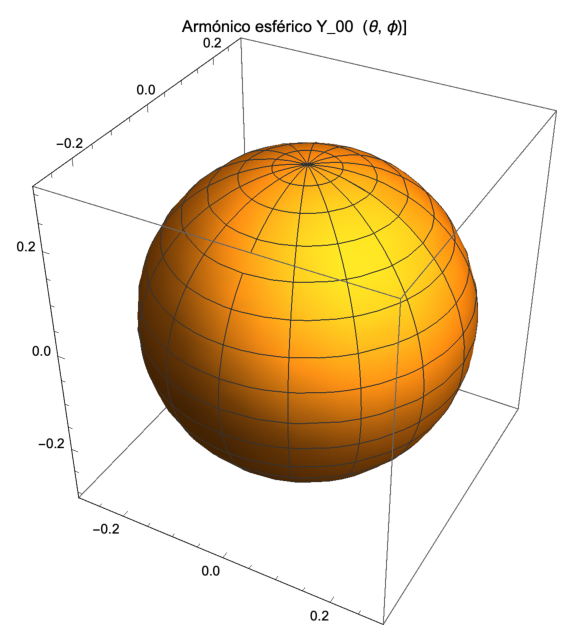
\includegraphics[scale=0.65]{Imagenes/Armonicos_Esfericos_00.eps}
\end{figure}
\end{frame}
\begin{frame}[plain]
\begin{figure}
    \centering
    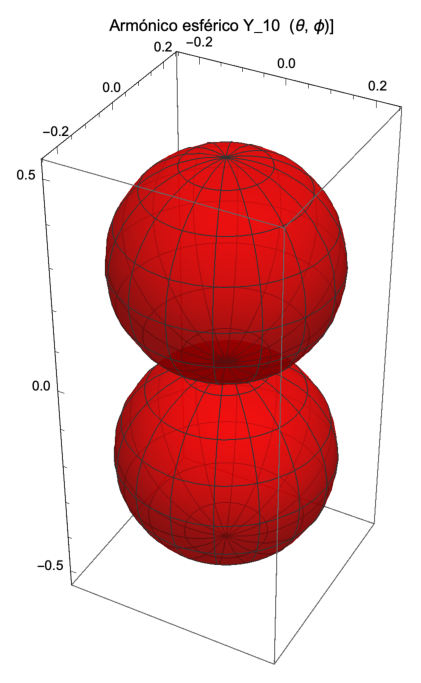
\includegraphics[scale=0.65]{Imagenes/Armonicos_Esfericos_10.eps}
\end{figure}
\end{frame}
\begin{frame}[plain]
\begin{figure}
    \centering
    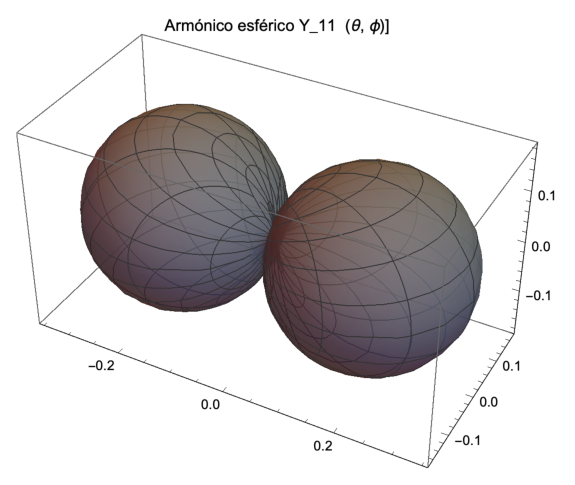
\includegraphics[scale=0.65]{Imagenes/Armonicos_Esfericos_11.eps}
\end{figure}
\end{frame}
\begin{frame}[plain]
\begin{figure}
    \centering
    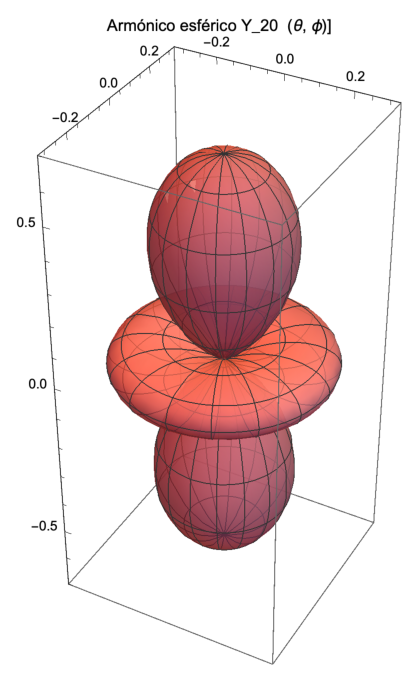
\includegraphics[scale=0.65]{Imagenes/Armonicos_Esfericos_20.eps}
\end{figure}
\end{frame}
\begin{frame}[plain]
\begin{figure}
    \centering
    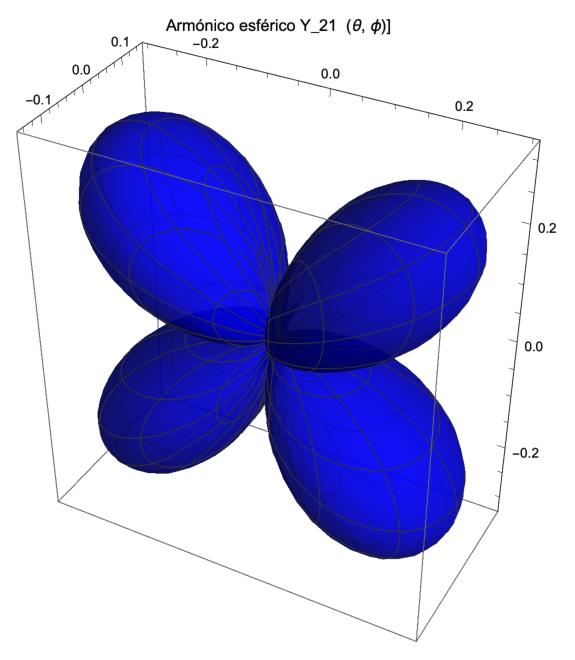
\includegraphics[scale=0.65]{Imagenes/Armonicos_Esfericos_21.eps}
\end{figure}
\end{frame}
\begin{frame}
\frametitle{Ortogonalidad de los armónicos esféricos}
Ya que contienen su $\theta$-dependiente de parte de la solución $P_{\ell}^{m}$ a la ecuación asociada de Legendre, \pause los $Y_{\ell}^{m}$ son mutuamente ortogonales cuando se integra de $-1$ a $+1$ sobre $d(cos \theta)$.
\end{frame}
\begin{frame}
\frametitle{Ortogonalidad de los armónicos esféricos}
Su ortogonalidad mutua respecto de $\phi (0 \leq \phi \leq 2 \pi)$ es aún más evidente. 
\\
\bigskip
\pause
El factor numérico en la ecuación (\ref{eq:ecuacion_045}) es elegido para hacer el $Y_{\ell}^{m}$ un conjunto ortonormal:
\end{frame}
\begin{frame}
\frametitle{Ortogonalidad de los armónicos esféricos}
Es decir:
\pause
\begin{equation}
\begin{aligned}[b]
\scaleint{6ex}_{-1}^{1} \scaleint{6ex}_{0}^{2 \pi} [ Y&_{\ell}^{m} (\theta, \phi) ]^{*} Y_{\ell'}^{m'} (\theta, \phi) d \phi d(\cos \theta) = \\[0.5em] 
&= \delta_{\ell \ell'} \delta_{m m'}
\end{aligned}
\label{eq:ecuacion_046}
\end{equation}
\end{frame}
\begin{frame}
\frametitle{Conjunto completo}
Adicionalmente, los armónicos esféricos forman un conjunto completo para cualquier función razonable de $\theta$ y $\phi$(como las que podemos encontrar en un problema físico).
\end{frame}
\begin{frame}
\frametitle{Conjunto completo}
La función puede expandirse como una suma de tales funciones:
\pause
\begin{equation}
f (\theta, \phi) = \nsum_{\ell=0}^{\infty} \nsum_{-\ell}^{\ell} a_{\ell m} \, Y_{\ell}^{m} (\theta, \phi)
\label{eq:ecuacion_047}
\end{equation}
\end{frame}
\begin{frame}
\frametitle{Conjunto completo}
Las constantes $a_{\ell m}$ están dadas por:
\pause
\begin{equation}
a_{\ell m} = \scaleint{6ex}_{-1}^{1} \scaleint{6ex}_{0}^{2 \pi} [ Y_{\ell}^{m} (\theta, \phi) ]^{*} f (\theta, \phi) \dd{\theta} \dd{(\cos \theta)}
\label{eq:ecuacion_048}
\end{equation}
\pause
Esto es una analogía exacta con una serie de Fourier y es un ejemplo particular de la propiedad general de soluciones de Sturm-Liouville.
\end{frame}

\end{document}